\documentclass[11pt]{standalone}
\usepackage[utf8]{inputenc}
\usepackage{amsmath}
\usepackage{amsfonts}
\usepackage{amssymb}
\usepackage{tikz}
\usetikzlibrary{patterns}
\begin{document}
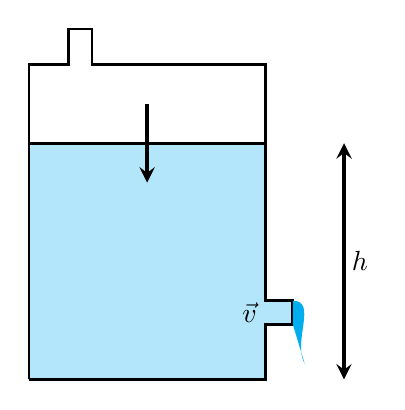
\begin{tikzpicture}[>=stealth]
\draw[line width=1pt] (0,3) -- (3,3);
\draw[line width=1pt] (0,0) -- (0,4) -- (0.5,4) -- (0.5,4.45) -- (0.8,4.45) -- (0.8,4) -- (3,4) -- (3,1) -- (3.35,1) -- (3.35,0.7) -- (3,0.7) -- (3,0) -- (0,0);
\draw[<->,line width=0.5mm] (4,0) -- (4,3);
\draw[fill=cyan!30,line width=1pt] (0,0) -- (0,3) -- (3,3) -- (3,1) -- (3.35,1) -- (3.35,0.7) -- (3,0.7) -- (3,0.7) -- (3,0) -- (0,0); 
\node at (2.8,0.85) [draw=none] (n3) {$\vec{v}$};
\draw[->,line width=0.5mm] (1.5,3.5) -- (1.5,2.5);
\fill[cyan=!30] (3.35,0.7) -- (3.35,1) to[in=120,out=0] (3.5,0.2);
\node at (4.2,1.5) [draw=none] (n2) {$h$};
\end{tikzpicture}
\end{document}